\documentclass[runningheads,a4paper]{llncs}
\usepackage[T1]{fontenc}
\usepackage{graphicx,booktabs,url,xurl}
\setlength{\emergencystretch}{3em}
\begin{document}
\title{Compiler-Guided Proof Repair in Lean 4: A Controlled Local-Model Pilot on Fixed Theorem Types}
\titlerunning{Controlled Lean 4 Proof Repair Pilot}
\author{Anonymous author}
\authorrunning{Anonymous author}
\institute{Author details withheld for publication-safety review}
\maketitle

\begin{abstract}
We compare no-repair generation (A), blind retry (B), and Lean-compiler-guided
repair (C) for English statements paired with fixed reviewed theorem types.
B and C start from identical failed candidates, use one hash-pinned 4-bit
Qwen2.5-7B instruction model, and allow at most three repair calls under common
context/output caps. Of 60 held-out statements, A verifies 0/60 and B 1/60;
C verifies 1/58 observed outcomes, with two unavailable outcomes. On the 58
complete paired trajectories, B and C each verify 1/58 (1.72\%): the paired
difference is 0.00 percentage points, with no discordant pairs. A degenerate
conditional bootstrap interval does not establish equivalence or account for
missingness. Full-cohort identification bounds are 0 to +3.33 points for C--B.
Counting unavailable C outcomes as failures yields the separately planned
1/60 sensitivity estimate. We report genuine outputs, compiler errors, resource
usage and failure cases rather than a demonstrated feedback benefit. One seed,
a three-case development pilot, low success, related families, author-assisted
AI review and privacy-limited public replay restrict the conclusions. The task
is fixed-type proof synthesis; autonomous NL-to-statement and end-to-end accuracy
are not measured.
\keywords{Lean 4 \and proof repair \and compiler diagnostics \and local inference \and negative results}
\end{abstract}

\section{Introduction and Research Questions}
An informal mathematical statement can be paired with a formal theorem type
yet still lack a proof accepted by a theorem prover. A generated proof may fail
because of syntax, unavailable names, type mismatches, an incomplete tactic
argument, or a mathematical mistake. A compiler supplies concrete evidence about
these failures, but additional generation alone may also repair them. A useful
comparison must distinguish diagnostic feedback from the benefit of more calls.

Our primary question is whether compiler-guided repair improves verified
success over equally budgeted blind repair, conditioned on the same initial
candidate. Secondary questions compare each repair condition with one-shot
generation and describe outcomes by initial error category. We do not assume
that feedback helps, or interpret a failure to reject as equivalence. The
experimental unit is a theorem trajectory, not an individual repair attempt.

The evaluated stage receives both English and a fixed AI-reviewed Lean type.
It therefore tests proof synthesis and repair within an NL-to-Lean workflow.
It does not measure unconstrained English-to-theorem translation, independent
semantic-review accuracy, or state-of-the-art mathematical problem solving.

\section{Related Work}
Lean 4 provides a dependently typed language and kernel-checked proof
infrastructure~\cite{demoura2021lean4}; Mathlib supplies the mathematical
library used here~\cite{mathlib2020}. Benchmarks such as
miniF2F~\cite{zheng2022minif2f} support formal theorem-proving evaluation,
while ProofNet studies paired informal and formal
mathematics~\cite{azerbayev2023proofnet}. LeanDojo studies tool-supported
theorem proving and retrieval~\cite{yang2023leandojo}. These settings motivate
careful separation of problem statements, proof generation, library access and
verification. Our experiment is a bounded paired comparison using a general
local instruction model. It includes no retrieval service, proof search tree,
fine-tuning, or paid hosted inference, and should not be compared directly with
systems using different tasks, data or compute budgets.

Compiler-conditioned repair training is studied by APRIL~\cite{wang2026april};
our study instead compares bounded inference retries with one unfine-tuned local
model. Work on faithfulness beyond compilation~\cite{zhang2026beyond} also
motivates distinguishing fixed-type proof success from semantic fidelity.

\section{System Architecture and Verification}
The pipeline loads immutable English/type pairs, renders an initial prompt,
generates one candidate, extracts the requested Lean block, and verifies it
against the fixed reference type. A and both repair branches share the exact
initial bytes and SHA-256. Each repair uses a fresh model conversation and
independent context-derived random stream. B receives the theorem, its current
candidate and fixed blind-feedback text. C receives the same template structure
with structured diagnostics from its immediately preceding failed compilation.
Neither branch receives the other branch's candidates or conversation.

The strict verifier rejects placeholder proofs and unauthorized declarations,
checks the exact elaborated theorem type, and inspects target axiom dependencies.
Only the standard \texttt{propext}, \texttt{Classical.choice} and
\texttt{Quot.sound} dependencies are accepted. A reference placeholder is used
only to compare types in a separate namespace; it is never counted as a target
proof, and a target depending on \texttt{sorryAx} is rejected. Compiler JSON,
source text, exit status, failure kind and elapsed time are stored. Compilation
proves neither the English interpretation nor the quality of explanatory prose.

Source-token and declaration guards run before compilation; axiom-policy
rejection can also occur afterward. Such events are not relabeled as compiler
errors. C stops if genuine candidate diagnostics are unavailable;
it is never supplied an invented compiler message. Timeouts, context-limit
failures and interrupted calls remain explicit missing/incomplete outcomes.

\section{Dataset, Provenance and Semantic Audit}
Starting from 96 prepared candidates, we exclude one exact duplicate and 20
nonduplicate records lacking adequate item-level provenance. The resulting 75
records comprise 16 textbook-derived statements~\cite{levin2021dmoi} and 59
adaptations of pinned formal-library statements. Citations, original source
bytes, license notices and item-level attribution are retained. Textbook
adaptations retain CC BY-SA 4.0 attribution; formal-library material retains
Apache-2.0 notices. These are evidence-based AI-assisted source assessments,
not invented publisher permissions or independent legal clearance.

Two original records were corrected: a positive-modulus premise was restored,
and ambiguous summation endpoints were made explicit. Both proofs were
reverified and both pairs were reviewed again with a separate Phi-4 model.
They remain excluded for source-provenance reasons; corrections were not used
to inflate eligible counts. Original records and before/after histories remain
available.

\begin{table}[t]
\centering
\caption{Frozen composition. Category, difficulty and provenance rows are separate partitions, not additive totals. Development/test occupy 5/54 curated families with no family overlap.}
\label{tab:dataset}
\small
\begin{tabular}{lrrr}
\toprule
Partition & Dev. & Test & Total \\
\midrule
Category: arithmetic identity & 2 & 11 & 13 \\
Category: divisibility & 3 & 17 & 20 \\
Category: induction & 6 & 8 & 14 \\
Category: inequality & 1 & 15 & 16 \\
Category: modular arithmetic & 3 & 9 & 12 \\
Difficulty: 1 & 2 & 2 & 4 \\
Difficulty: 2 & 10 & 57 & 67 \\
Difficulty: 3 & 2 & 1 & 3 \\
Difficulty: 4 & 1 & 0 & 1 \\
Textbook / CC BY-SA 4.0 & 8 & 8 & 16 \\
Formal library / Apache-2.0 & 7 & 52 & 59 \\
Total unique statements & 15 & 60 & 75 \\
\bottomrule
\end{tabular}
\end{table}


The approved replacement policy uses explicit AI adjudication of quantifiers,
domains, assumptions, strength, endpoints and equivalent encodings. Phi-3.5 and
Phi-4 audit responses are retained, including schema failures and unsupported
objections. The authoring coding assistant adjudicated the exact selected pairs
using candidate-specific mathematical comparisons and reference evidence. It
is not author-independent human review. An uncertain or unfaithful final
adjudication is inadmissible; unreliable raw AI output is not a faithful vote.

The independent reviewer models were demonstrably fallible: for example, one
claimed that $1(1+1)$ was odd. Exact arithmetic refutes that alleged
counterexample. Generic placeholders, hallucinated hypotheses and proof-method
confusion were separately flagged. All 96 original reference types have strict
Lean evidence; handwritten bounded probes cover 26,467 accepted finite
assignments, with 88 exact predicates and eight approximate numerical probes.
These checks supplement, rather than establish, English equivalence.

Whole binomial, linear-solvability and modular-power families were grouped before
primary-model test access. No curated family crosses splits. The 15 development
statements occupy five conservative family clusters; the 60 test statements
occupy 54. These are not claimed to be 75 independent topic families.
All texts were accessed for authorized curation, but no held-out primary-model
proof outcome was used to select prompts or settings. Ordered IDs and exact
dataset bytes were frozen with cryptographic hashes. The source commit and local
launch record precede held-out inference. No evidence establishes public publication
of the IDs/hash before testing; this is an internal freeze, not external preregistration.

\section{Frozen Experimental Design}
The primary model is \texttt{mlx-community/Qwen2.5-7B-Instruct-4bit}, run
offline with MLX~\cite{qwenmlx,mlxlm}. Its immutable converted snapshot is
\path{c26a38f6a37d0a51b4e9a1eb3026530fa35d9fed}. Inventory hashes bind all weights, tokenizer files and
the native chat template. Quantization is 4-bit with group size 64. MLX 0.32.4,
MLX-LM 0.32.2 and Transformers 5.21.0 are recorded. Decoding uses temperature
0.2, top-$p$ 1, at most 2,000 output tokens and an 8,192-token total context cap.
One primary seed, 2027, is used; three-seed robustness is not claimed.
The local host uses an Apple M4 processor with 16 GiB physical memory.

The per-call seed is the first unsigned 32-bit word of SHA-256 of the base
seed, phase/problem/condition/step context and exact prompt hash. Consequently,
B's stopping behavior does not shift C's random stream. All conditions use
the same model and environment. The common caps are a prompt budget, not equal
realized input-token cost: genuine C diagnostics lengthen prompts, and one C
prompt exceeds the cap before generation. A token-cost-matched effect is not measured. A has zero repairs; B and C each permit up to
three, with at most seven logical generation intents per problem including the shared
initial call. Success stops a branch. Model weights are released during the
memory-heavy Lean check and reloaded from the same verified bytes on the next
call. This preserves independent KV state and incurs measurable loading overhead.

Exploratory development pilots exposed Lean 3-style syntax and high resident
memory cost. Before any held-out generation, the final protocol added the same
explicit Lean 4 syntax instruction to all three conditions and fixed the memory
schedule. This was syntax/implementation development, not test-outcome tuning;
the format diagnostic still failed mathematical verification. Prototypes are
preserved and excluded from study estimates. The final pilot covers only three of the fifteen development cases and passed
the provenance/control audit, and an actual resume invocation generated no new
calls. No model, prompt, dataset or budget changed after held-out execution began.

Conditions execute B before C rather than in randomized order. Each call has a
durable intent, raw response and token stream; each verification and branch
transition has a checkpoint. Resume reuses completed outputs. An incomplete
generation intent consumes its logical call and is not silently regenerated.
The environment is Lean 4.32.0 with clean Mathlib commit
\path{81a5d257c8e410db227a6665ed08f64fea08e997}. There is no provider fallback or paid inference path.

\section{Results and Statistical Analysis}
Table~\ref{tab:abc} distinguishes observed outcomes from missingness. A succeeds
0/60 (0.00\%); B succeeds 1/60 (1.67\%); C succeeds 1/58 observed outcomes
(1.72\%), with 57 known failures and two unavailable outcomes. Wilson intervals
are [0.00,6.02]\% for A, [0.29,8.86]\% for B, and [0.31,9.14]\% for observed C.
They assume independent problem units; related family clusters limit that assumption.

\begin{table}[t]
\centering
\caption{A/B/C observed outcomes and known completed-response resources. C has two unavailable outcomes; its primary observed rate is 1/58. Repair means use the 60 eligible-case denominator, including zero completed repairs. Resource totals include the shared initial in each counterfactual row.}
\label{tab:abc}
\small
\begin{tabular}{lrrrr}
\toprule
Condition & Verified/observed & Missing & Rate & Wilson 95\% \\
\midrule
A & 0/60 & 0 & 0.00\% & [0.00, 6.02] \\
B & 1/60 & 0 & 1.67\% & [0.29, 8.86] \\
C & 1/58 & 2 & 1.72\% & [0.31, 9.14] \\
\bottomrule
\end{tabular}
\par\vspace{4pt}
\begin{tabular}{lrrrr}
\toprule
Cond. & Repairs (mean) & Tokens in/out & Call wall s & Lean s \\
\midrule
A & 0 (0.00) & 12,929/27,862 & 1908.6 & 2361.9 \\
B & 178 (2.97) & 122,029/83,485 & 8120.5 & 8923.9 \\
C & 172 (2.87) & 252,935/74,778 & 9870.8 & 8906.3 \\
\bottomrule
\end{tabular}
\par\vspace{4pt}
\begin{minipage}{.98\linewidth}\footnotesize
Initial success is 0/60. On the 58 complete B/C pairs each method succeeds once: paired difference 0.00 percentage points. B consumes 178 logical repair intents; C consumes 174, of which 172 complete. Sensitivity counting missing C as failure is 1/60 (1.67\%), not the observed C rate. Call wall times exclude the unavailable response and preflight rejection; they are not full-run cost estimates.
\end{minipage}
\end{table}


\subsection{Matched effects and uncertainty}
On 58 complete pairs, B and C each succeed on the same single target,
\texttt{lib\_a\_exp\_add}. The C--B risk difference is 0.00 percentage points,
with zero discordant pairs. The conventional exact two-sided McNemar value is $p=1.0$ with
zero discordant pairs. This does not establish equivalence. Both problem and family-cluster
bootstrap intervals are [0.00,0.00] points, conditional on those observed pairs.
This degeneracy reflects identical observed outcomes, not high precision about
a general feedback effect.

\begin{center}\begin{minipage}{\linewidth}
\centering
\textbf{Paired success differences in percentage points; conventional exact McNemar p=1.0 for zero discordance. Cluster bootstrap is primary; paired-score bounds are an independent-pair sensitivity, not equivalence bounds.}\par\vspace{3pt}
\small
\resizebox{\linewidth}{!}{%
\begin{tabular}{llllll}
\toprule
Contrast & Pairs & Diff. pp & Cluster 95\% pp & Score 95\% pp & Exact p \\
\midrule
C\_minus\_B & 58 & +0.00 & [+0.00, +0.00] & [-6.83, +6.83] & 1.0 \\
C\_minus\_A & 58 & +1.72 & [+0.00, +5.56] & [-4.65, +9.14] & 1.0 \\
B\_minus\_A & 60 & +1.67 & [+0.00, +5.45] & [-4.50, +8.86] & 1.0 \\
\bottomrule
\end{tabular}}
\end{minipage}\end{center}


The revised paired point estimates, intervals and tests use the same complete
cases for each contrast. For C--A this is 58 pairs (difference +1.72 points);
for B--A it is 60 (+1.67 points). Both exact $p$ values and Holm-adjusted values
are 1. The three planned comparisons remain in Holm multiplicity accounting,
including the conventional $p=1.0$ for zero-discordance C--B. Bootstrap sensitivity uses 10,000 resamples and
seed 20271021. The complete C contrasts have 52 represented family clusters;
the full test cohort has 54. Resampling cases or families does not remove
selection bias from unavailable outcomes. No statistically supported improvement
is claimed; low success and only one solved target give limited power.

% POST_HOC_CALIBRATION_BEGIN
\paragraph{Post-hoc calibration.} A separately labeled analysis uses Newcombe's paired method 10~\cite{newcombe1998paired}: Wilson marginal score intervals with an adjusted phi coefficient. For the 58 C--B pairs this sensitivity interval is [-6.83, +6.83] percentage points. It assumes independent pairs and is not a replacement for family-cluster sensitivity; related families and unavailable outcomes limit inference. The degenerate empirical bootstrap does not rule out these larger effects. Full post-hoc method and power-assumption tables are provided separately.
% POST_HOC_CALIBRATION_END

\subsection{Unavailable outcomes and sensitivity}
The frozen protocol explicitly planned both complete-pair inference and a
full-denominator missing-as-failure sensitivity. The latter is C=1/60 (1.67\%),
with Wilson interval [0.29,8.86]\%, and is not the observed C rate. Both missing
C cases failed in B. If neither missing C outcome would succeed, the full-cohort
C--B difference is zero; if both would succeed it is +3.33 percentage points.
These are identification bounds, not confidence limits. The zero bootstrap
interval does not cover this missingness uncertainty.

For \texttt{lib\_a\_trig\_unit}, the exact C1 prompt has 9,653 input tokens,
already exceeding the 8,192-token context cap before reserving 2,000 output
tokens. The recorded preflight rejection produced no response. For
\texttt{lib\_i\_bernoulli}, C1 has 2,205 input tokens but only a stream header
survives, with zero durably observed generated tokens. No candidate is available
to verify. The terminal no-replay rule forbids either retry; changing diagnostics,
caps or the seed would change the frozen study. The interruption cause is unknown.

\begin{figure}[t]
\centering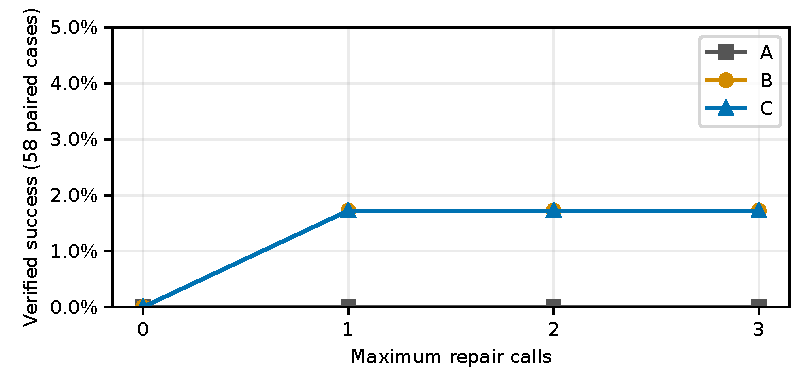
\includegraphics[width=.9\linewidth]{generated/review_v2/success_budget.pdf}
\caption{Verified success versus allowed repair calls on the same 58 complete
trajectories for all curves and budgets. B and C overlap. The displayed axis is
0--5\%. The two unavailable C trajectories are excluded at every budget; this
complete-case display does not assume they are missing at random.}
\label{fig:budget}
\end{figure}

\subsection{Attempts, tokens and latency}
The ledger contains 412 logical generation intents and 410 completed responses:
60 shared initial outputs, 178 B repairs and 172 C repairs. C has 174 repair
intents, including its preflight rejection and header-only interruption. An
intent is not a confirmed completed inference call. B completes a mean 2.97
repairs per eligible problem; C completes 2.87 (2.90 consumed intents). Both
repair-count medians are three. Physical completed-call totals count the shared
initial once: 362,035 input tokens, 130,401 output tokens and 11,233.6 native
generation seconds. Counterfactual condition rows each include their initial.
No unavailable response tokens or duration are invented.

\begin{center}\begin{minipage}{\linewidth}\centering
\textbf{Known completed-response resource distributions. Loading is included in call wall time. These are calls, not independent theorem observations. Missing response costs are not imputed.}\par\vspace{3pt}
\small
\begin{tabular}{llrrr}
\toprule
Cond. & Measure & Calls & Mean & Median \\
\midrule
A & Input tokens & 60 & 215.5 & 215.0 \\
A & Output tokens & 60 & 464.4 & 198.0 \\
A & Call wall s & 60 & 31.8 & 16.3 \\
A & Generation s & 60 & 27.2 & 11.8 \\
B & Input tokens & 238 & 512.7 & 369.0 \\
B & Output tokens & 238 & 350.8 & 172.5 \\
B & Call wall s & 238 & 34.1 & 16.9 \\
B & Generation s & 238 & 26.1 & 12.3 \\
C & Input tokens & 232 & 1090.2 & 968.0 \\
C & Output tokens & 232 & 322.3 & 170.5 \\
C & Call wall s & 232 & 42.5 & 21.0 \\
C & Generation s & 232 & 28.7 & 16.6 \\
\bottomrule
\end{tabular}
\end{minipage}\end{center}

\begin{center}\begin{minipage}{\linewidth}\centering
\textbf{Resources per theorem on the same 58 complete pairs (230 completed calls per condition, including the shared initial). Observed costs are descriptive; B-before-C order and shared-host activity prevent a causal speed claim.}\par\vspace{3pt}
\small
\begin{tabular}{lrrr}
\toprule
Cond. & Mean tokens in/out & Wall s mean/median & Mean generation s \\
\midrule
B & 1980.9/1336.2 & 131.7/68.6 & 99.6 \\
C & 4353.5/1249.2 & 167.9/84.8 & 112.5 \\
\bottomrule
\end{tabular}
\end{minipage}\end{center}


Call wall time includes model loading; native generation time excludes it.
The table reports completed-response costs only, not unknown full-run costs.
Sequential B-before-C execution, cache state and an observed unrelated MLX
workload confound causal latency comparisons. Recovery elapsed time includes an
inactive interval and is not continuous compute. The diagnostic input overhead
also prevents reading this as an equal-total-token-cost comparison.
\section{Compiler-Error Taxonomy}
Table~\ref{tab:errors} uses the frozen deterministic primary taxonomy: parser
errors take precedence, then unknown names, type/elaboration errors, tactic/goals,
and other errors. Each failed initial belongs to one group. It includes 26 parser,
20 unknown-name, nine tactic/goal, four type/elaboration and one other failure.
The only solved target is in the unknown-name group (B=C=1/20 there); all other
groups have zero observed repairs that verify. C is unavailable in one parser
and one tactic/goal case, so their observed denominators are 25 and eight.
These descriptive counts do not support error-specific superiority claims.

\begin{table}[t]
\centering
\caption{Primary initial-error taxonomy and observed repair success fractions. Categories are pre-specified and mutually exclusive; denominators are observed B/C outcomes within each group. Groups below five cases remain descriptive.}
\label{tab:errors}
\small
\begin{tabular}{lrrrr}
\toprule
Initial error & Cases & B solved/obs. & C solved/obs. & C missing \\
\midrule
Other & 1 & 0/1 & 0/1 & 0 \\
Parser/syntax & 26 & 0/26 & 0/25 & 1 \\
Tactic/goals & 9 & 0/9 & 0/8 & 1 \\
Type/elaboration & 4 & 0/4 & 0/4 & 0 \\
Unknown name & 20 & 1/20 & 1/20 & 0 \\
\bottomrule
\end{tabular}
\end{table}

\begin{figure}[t]
\centering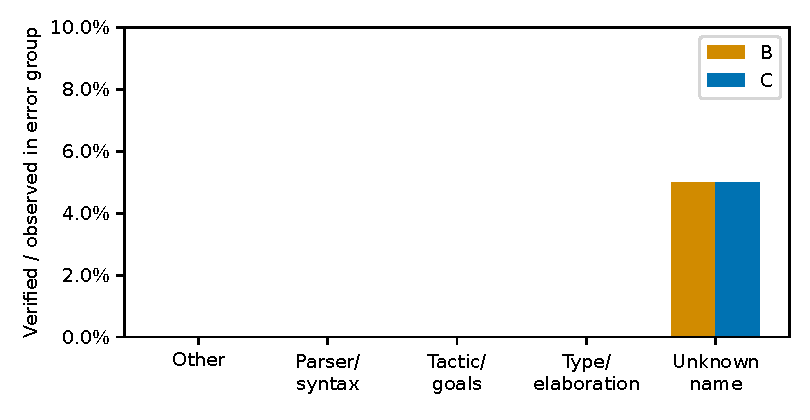
\includegraphics[width=.9\linewidth]{generated/review_v2/error_rates.pdf}
\caption{Observed repair-success fractions by primary initial error. B/C use
their observed denominators in Table~\ref{tab:errors}; the two missing C outcomes
remain explicit. No subgroup hypothesis tests are added.}
\label{fig:errors}
\end{figure}

Representative diagnostics identify unavailable symbols, malformed syntax,
ill-typed applications and unsolved proof obligations. Such messages identify an
obstacle but do not supply a correct mathematical argument or a working lemma.
Unknown identifiers and unknown theorem names are not reliably distinguishable
from compiler wording alone; tactic and unsolved-goal messages can co-occur.
A separate, explicitly post-hoc message-tag artifact records these overlapping
subtypes and genuine examples, without replacing the pre-specified primary groups.
No compiler timeout was observed among the completed candidates; the context
rejection is a generation resource failure, not a Lean error. Failed model
outputs and their actual diagnostics remain retained, including repeated errors.

% POST_HOC_PROCESS_BEGIN
\subsection{Exploratory process diagnostics}
The following measurements were defined after observing the original outcomes
and do not alter the frozen success analysis. B repeated the immediately preceding
candidate in 90/178 completed repairs, C in 70/172. Whole-family resampling,
10,000 draws and seed 20271021, preserves repair and family dependence.
The exploratory C--B repetition difference is -9.86 percentage points
(95\% family-bootstrap interval [-19.77,-0.50]). This is one of several post-hoc
contrasts, not a confirmatory diagnostic-use test or a proof-success improvement.
At least one preceding unknown name disappears in B 12/76 eligible repairs and
C 14/70; B's diagnostics are used by the analyst only. Syntactic name removal,
edit distance, fewer messages and category transitions are not certified fixes.
Character/token edits, grayscale transition matrices, prompt-length distributions,
and assumption-based power calculations are provided as post-hoc supplementary
artifacts. No new held-out inference, replay or outcome imputation occurs.
% POST_HOC_DEV_BEGIN
\paragraph{Exploratory development placebo.} A separately frozen post-hoc control used fresh shared initials on 15 development problems, one seed, three repair arms and only genuine different-problem/family donor diagnostics. Only diagnostic filename metadata was normalized consistently; compiler-message content remained unchanged. Observed verified outcomes were A: 0/15, B: 0/15, C: 0/15, C\_placebo: 0/15. Completed-repair counts were C repetition 23/45, own-name removal 3/19; C\_placebo repetition 32/45, own-name removal 2/17. The observed higher own-name removal and lower repetition under real diagnostics are consistent with diagnostic-content sensitivity. This exploratory one-seed pattern does not prove that the model uses diagnostic content. Five dev families, independent condition RNG streams, donor category/length matching and sequential execution limit inference; no hypothesis-test or proof-of-use claim is made.
% POST_HOC_DEV_END
% POST_HOC_PROCESS_END

\section{Qualitative Repair Cases}
Five authentic cases were selected post hoc for outcome, category and error
coverage. There is only one distinct solved test target; five successes are not
claimed. Each example displays the actual immediately preceding candidate,
its real compiler message, and the last recorded repair. A blind case's compiler
message is shown for analysis only: B did not receive it. Excerpts are limited
to five lines and 58 characters per line, with ASCII display transliteration;
full original candidate bytes and hashes remain in the evidence. A byte-identical
retry is a genuine observed non-change, not a manufactured repair.
\paragraph{lib\_a\_exp\_add (B).}
For all real x and y, exp(x+y)=exp(x)*exp(y).
Actual last repair: B1; Lean success: True. Candidate is different candidate bytes; success is determined by Lean, not the edit itself.
First actual changed text: removed [have h : Real.exp (x + y) = Real.ofReal (Real]; inserted [].
Immediately preceding genuine diagnostic: Unknown constant `Real.ofReal`.
The blind model did not receive this diagnostic.
\textit{Before (display-only excerpt):}
\begin{verbatim}
open scoped BigOperators
theorem study_a_exp_add (x y : Real) : Real.exp (x + y) =
:= by
  have h : Real.exp (x + y) = Real.ofReal (Real.exp x * Re
    rw [Real.exp_add]
\end{verbatim}
\textit{After (display-only excerpt):}
\begin{verbatim}
open scoped BigOperators
theorem study_a_exp_add (x y : Real) : Real.exp (x + y) =
:= by
  rw [Real.exp_add]
\end{verbatim}
\paragraph{div\_007 (C).}
For all integers a and b, if a and b are even, then a + b is even.
Actual last repair: C3; Lean success: False. Candidate is byte-identical to its predecessor.
No text changed in this actual retry.
Immediately preceding genuine diagnostic: Unknown identifier `even\_add`.
C received this predecessor diagnostic in its structured feedback.
\textit{Before (display-only excerpt):}
\begin{verbatim}
theorem even_add_of_even (a b : Int) (ha : Even a) (hb : E
by
  obtain <a', ha'> := ha
  obtain <b', hb'> := hb
  exact even_add ha' hb'
\end{verbatim}
\textit{After (display-only excerpt):}
\begin{verbatim}
theorem even_add_of_even (a b : Int) (ha : Even a) (hb : E
by
  obtain <a', ha'> := ha
  obtain <b', hb'> := hb
  exact even_add ha' hb'
\end{verbatim}
\paragraph{lib\_a\_trig\_unit (B).}
For every real x, sin(x)\textasciicircum{}2+cos(x)\textasciicircum{}2 equals one.
Actual last repair: B3; Lean success: False. Candidate is different candidate bytes; success is determined by Lean, not the edit itself.
First actual changed text: removed [Real.sin x * Real.sin x + Real.cos x * Real.c]; inserted [(Real.sin x) * (Real.sin x) + (Real.cos x) * ].
Immediately preceding genuine diagnostic: unsolved goals
x : Real
|- 1 = Real.sin x * Real.sin x + Real.cos x * Real.cos x.
The blind model did not receive this diagnostic.
\textit{Before (display-only excerpt):}
\begin{verbatim}
open scoped BigOperators
theorem study_a_trig_unit (x : Real) : (Real.sin x) ^ 2 +
:= by
  have h1 : (Real.sin x) ^ 2 + (Real.cos x) ^ 2 = Real.sin
    simp
\end{verbatim}
\textit{After (display-only excerpt):}
\begin{verbatim}
open scoped BigOperators
theorem study_a_trig_unit (x : Real) : (Real.sin x) ^ 2 +
:= by
  have h1 : (Real.sin x) ^ 2 + (Real.cos x) ^ 2 = (Real.si
    simp
\end{verbatim}
\paragraph{div\_008 (C).}
Prove that for all integers n, it is the case that n is even if and only if 3n is even. That is, prove both implications: if n is even, then 3n is even, and if 3n is even, then n is even.
Actual last repair: C3; Lean success: False. Candidate is different candidate bytes; success is determined by Lean, not the edit itself.
First actual changed text: removed [\_]; inserted [(by rw [mul\_one, hk, mul\_one])].
Immediately preceding genuine diagnostic: Tactic `split` failed: Could not split an `if` or `match` expression in the goal

Hint: If you meant to destruct this structure, use the `cases` tactic instead

Hint: Use `set\_opti.
C received this predecessor diagnostic in its structured feedback.
\textit{Before (display-only excerpt):}
\begin{verbatim}
theorem even_iff_even_three_mul (n : Int) : Even n <-> Eve
by
  split
  ? intro h
    obtain <k, hk> := h
\end{verbatim}
\textit{After (display-only excerpt):}
\begin{verbatim}
theorem even_iff_even_three_mul (n : Int) : Even n <-> Eve
by
  split
  ? intro h
    obtain <k, hk> := h
\end{verbatim}
\paragraph{div\_011 (C).}
For integers a, b, and c, if a divides both b and c, then a divides both b + c and b - c.
Actual last repair: C3; Lean success: False. Candidate is byte-identical to its predecessor.
No text changed in this actual retry.
Immediately preceding genuine diagnostic: Type mismatch
  k + l
has type
  Int
of sort `Type` but is expected to have type
  a  |  b + c
of sort `Prop`.
C received this predecessor diagnostic in its structured feedback.
\textit{Before (display-only excerpt):}
\begin{verbatim}
theorem dvd_add_sub_int (a b c : Int) (hab : a  |  b) (hac
:= by
  obtain <k, hk?> := hab
  obtain <l, hl?> := hac
  exact <k + l, k - l, by
\end{verbatim}
\textit{After (display-only excerpt):}
\begin{verbatim}
theorem dvd_add_sub_int (a b c : Int) (hab : a  |  b) (hac
:= by
  obtain <k, hk?> := hab
  obtain <l, hl?> := hac
  exact <k + l, k - l, by
\end{verbatim}

\section{Semantic Faithfulness and Threats to Validity}
\begin{table}[t]
\centering
\caption{AI-assisted reference faithfulness, not autonomous translation accuracy or human-gold accuracy. Original 96-item labels precede correction, source exclusion and final adjudication.}
\label{tab:semantic}
\small
\begin{tabular}{lrrl}
\toprule
Evidence population & Faithful & Not faithful & Uncertain/invalid \\
\midrule
Coding-AI original references (96) & 94 & 1 & 1 uncertain \\
Phi-4 original responses (96) & 72 & 11 & 13 invalid \\
Selected AI-eligible references (75) & 75 & 0 & 0 uncertain \\
Independent human labels & 0 & 0 & Not measured \\
\bottomrule
\end{tabular}
\end{table}

Historical coding-AI assessments label 94 original references faithful, one
not faithful, and one uncertain. The unfaithful example, \texttt{mod\_001},
omits the English positive-modulus restriction in Lean; the uncertain example,
\texttt{ind\_001}, leaves summation endpoints ambiguous. Both were corrected
and rechecked, but remain excluded for source provenance. Twenty nonduplicate
source-insufficient items and one exact duplicate are excluded overall. Selected
75/75 faithful AI adjudications are eligibility decisions, not measured accuracy.
The reference-review labels are not model-generated statement translations;
autonomous Stage-A and end-to-end semantic accuracy are not measured.

Successful proofs must have the exact reviewed reference type; changing a
quantifier, adding a hypothesis or weakening the conclusion cannot substitute
for solving that target. Nevertheless, faithfulness to English remains
conditional on the AI-adjudicated reference. We report review coverage and
provenance, not independently measured semantic accuracy. No AI output is
represented as an independent human judgment.

The authoring/adjudicating assistant can share systematic biases with the
dataset construction process. Separate Phi reviewers were unreliable, and
bounded mathematical probes are not exhaustive proofs of informal meaning.
Source/library exposure and direct named-lemma reuse may affect performance;
the dataset is not a contamination-free benchmark. Curated family boundaries
are mathematical judgments, not guarantees of statistical independence. The
development set has only five family clusters, and results use one model,
one quantization, one primary seed and one local hardware setting. The model's
knowledge can predate the pinned Lean/Mathlib interfaces. Fixed call and context
caps can stop repair without exhausting mathematical possibilities. These
limits preclude broad claims about compiler feedback, larger models or
unrestricted NL-to-formal translation.

\section{Reproducibility and Authorization Provenance}
All results derive from the frozen protocol and ordered dataset, with durable
raw generations, compiler JSON, exact sources, token counts, timings, failures
and resume checkpoints. Protocol SHA-256 is
\path{a032110d7afbc367c2daa820bd17511c6ff5dba2d1164e0130ea5d1c4b693317}; dataset-freeze SHA-256 is
\path{de0850197b821ca4c519737c4cffb16d78e2a329d15be6c7f3c6a7f5487db67f}; model inventory SHA-256 is
\path{24d68abbe5e1434e5263ad123cca517c2c1799c7465e104e83f6cb02baeac4f9}. The pre-held-out source commit and launch time,
source/evidence hashes and a release build manifest accompany the review bundle.
Original complete test logs and historical exploratory evidence remain local.
The original reference batch was freshly recompiled, and both successful model
candidates were reverified against the exact targets and allowed axioms.
Reconstruction checks every completed token journal against its raw response,
re-tokenizes all prompts offline, and regenerates metrics deterministically.
Raw-evidence whitespace is preserved; editable source whitespace is checked separately.

The student reported supervisor approval of AI-assisted semantic review and
free local MLX substitution on 28 October 2026. The original decision date,
document and signature were not supplied; approval is not claimed independently
verified. Exact implementation choices were frozen under the user's execution
authorization. No publisher permission or human review was fabricated. AI tools
assisted construction, adjudication and inference; they are not credited as
authors. Author identity and correspondence are withheld in this publication-safety review copy.

Public evidence is a privacy-redacted view. Paths inside compiler diagnostics,
prompts and metadata are replaced in exported copies; recorded original hashes,
token counts and seeds still describe the original private bytes. The original
frozen validators must not be applied to redacted views as though their bytes
were identical. Aggregate reanalysis is public; exact prompt replay and complete
source-evidence validation require the preserved originals. This is a disclosed
public reproducibility limit, not a replacement or revision of the experiment.

\section{Conclusion}
This internally frozen, single-seed empirical pilot records a controlled local comparison of one-shot, blind and
compiler-guided proof repair for 60 fixed theorem targets with shared initial
candidates. The recorded experiment does not establish a robust advantage for compiler feedback; a non-significant test is not evidence of equivalence. The contribution is the hash-committed paired evidence
and its failure analysis under a clearly delimited low-resource configuration,
not a claim of general superiority, equivalence, independent human semantic validation, or
complete unconstrained natural-language formalization.

\bibliographystyle{splncs04}
\bibliography{references}
\end{document}
